\subsection{Diseño de la interfaz}

Como se ha mencionado en el apartado \emph{Especificación de requisitos de la interfaz}\ref{especificacion-interfaz}, la aplicación se compone de una única pantalla, basada en scroll vertical, que se irá adapando a la acción que en cada momento se requiera al usuario.

Sobre ella serán cargando los paneles que se encarguen de la interacción \emph{usuario - máquina}.

En todo momento se ha perseguido hacer una interfaz en torno a la ``simpleza'' de uso y manejo de la aplicación, evitando controles, configuraciones y combinaciones que pudieran generar confusión.

A continuación se presentan los diseños de los paneles de la aplicación. Sendos paneles pueden verse recogidos en las imágnes de diseño \ref{fig:diseno-panales}.

\subsubsection{Panel de selección de género musical}

En la figura \ref{fig:pantalla-seleccion} se muestra cómo quedaría el panel de selección musical maquetado.

% \begin{figure}[H]
% \begin {center}
%     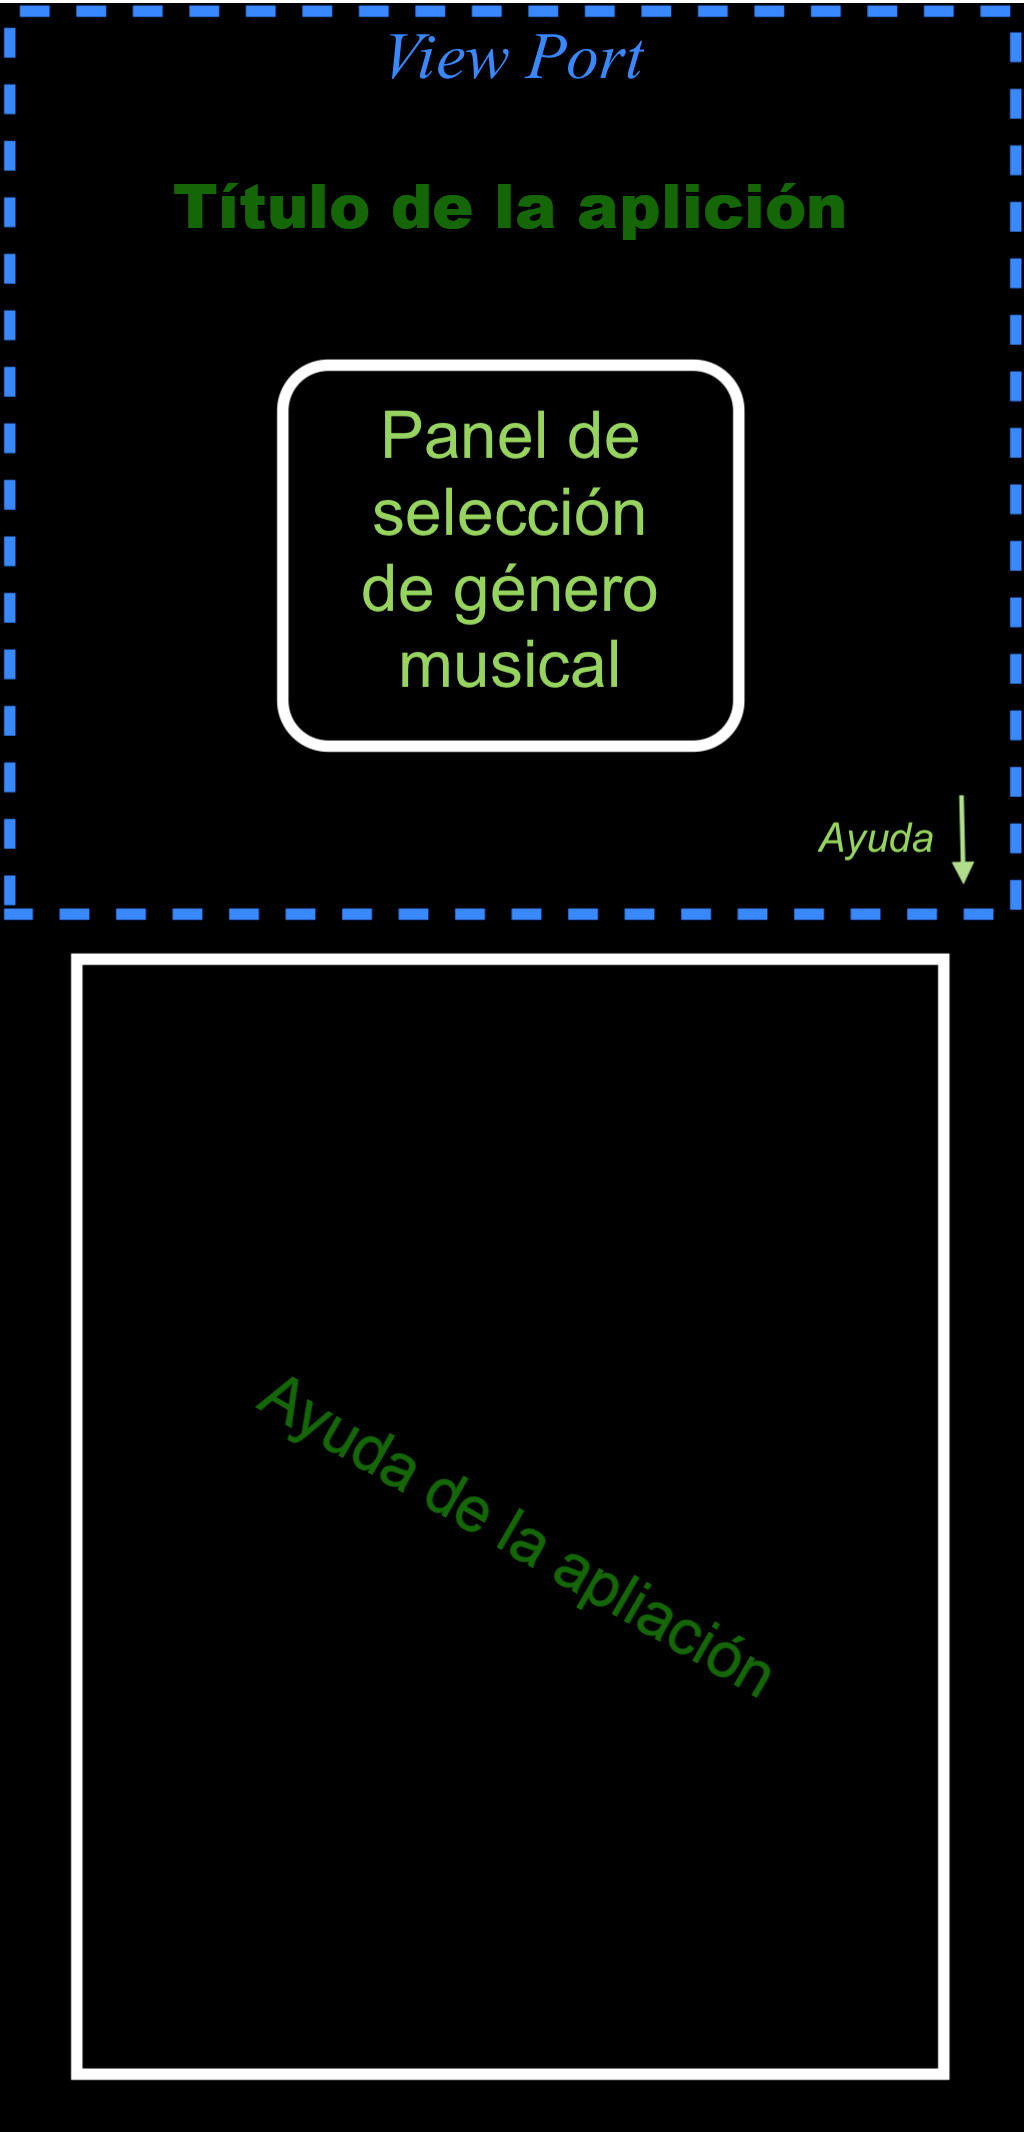
\includegraphics[width=0.35\textwidth]{images/panel_seleccion.png}
%         \caption{Pantalla de selección de género musical.}
% \end {center}
% \label{fig:pantalla-seleccion}
% \end{figure}

Este panel albergará los siguientes items nombrados anteriormente en la especificación de la interfaz:

\begin{itemize}
    \item Una lista de géneros musicales para seleccionar.
    \item Un botón para instar la creación de una pieza musical del género seleccionado.
    \item Un botón para dirigirse a la zona de ayuda de la ventana.
\end{itemize}

La interacción con el panel de selección de género musical dará paso al siguiente estado de la pantalla.

El bobón ayuda estará presente durante todo el ciclo de vida del software, haciendo que el scroll se desplace verticalmente, provocando que el \emph{View port} se mueva verticalmente y se pueda consultar el contenido de la ayuda
 
\subsubsection{Panel de de descarga y valoración}

La figura \ref{fig:pantalla-descarga} muestra el diseño del panel que aparecerá como consecución de la solicitiud de una pieza musical. Permitirá descargar la pieza musical generada y emitir una valoración de la misma.

% \begin{figure}[H]
%     \begin {center}
%         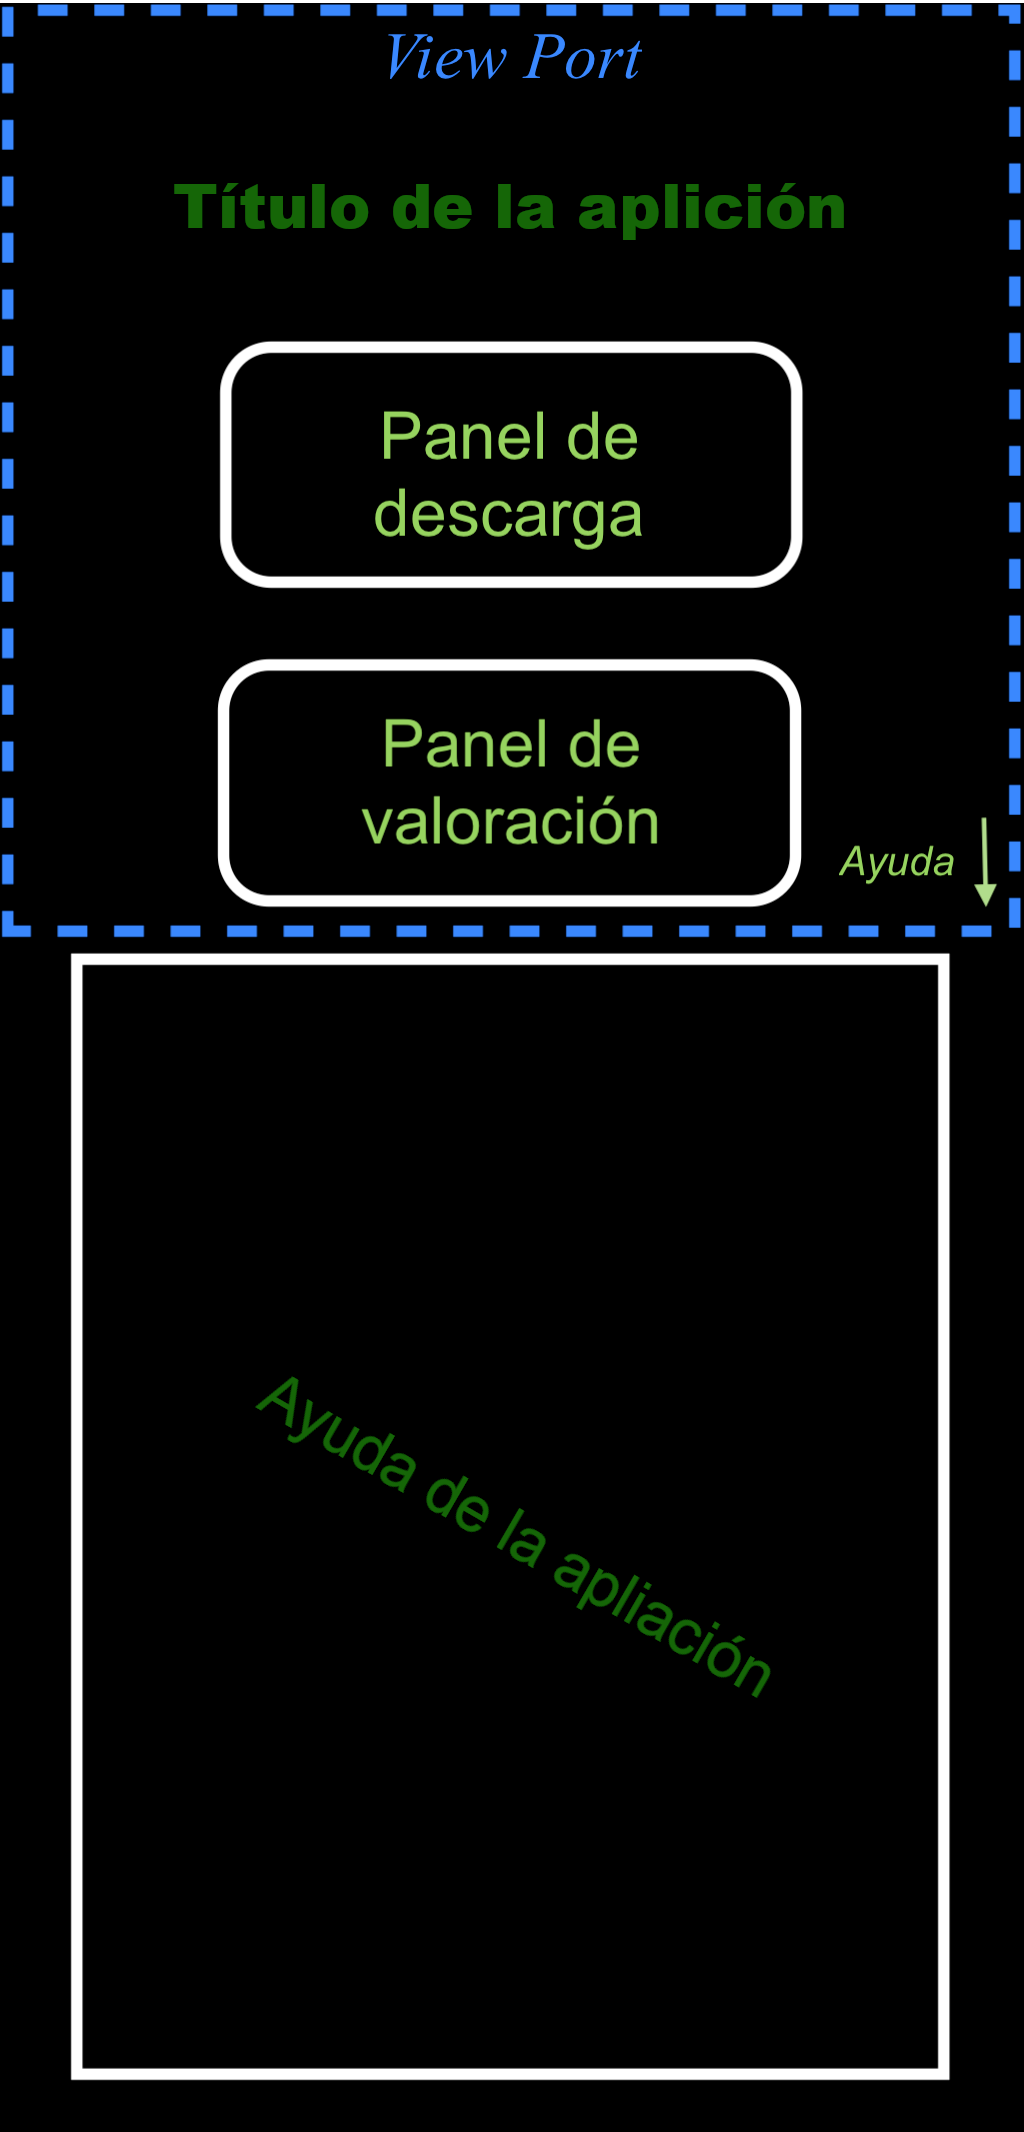
\includegraphics[width=0.35\textwidth]{images/panel-descarga-valoracion.png}
%             \caption{Pantalla de descarga y valoración.}
%     \end {center}
%     \label{fig:pantalla-descarga}
%     \end{figure}

Al igual que en el panel anterior, el botón de ayuda estará visible e interactuable.

\begin{figure}[H]
    \begin{center}
      \subfigure[Pantalla de selección de género musical.]{
        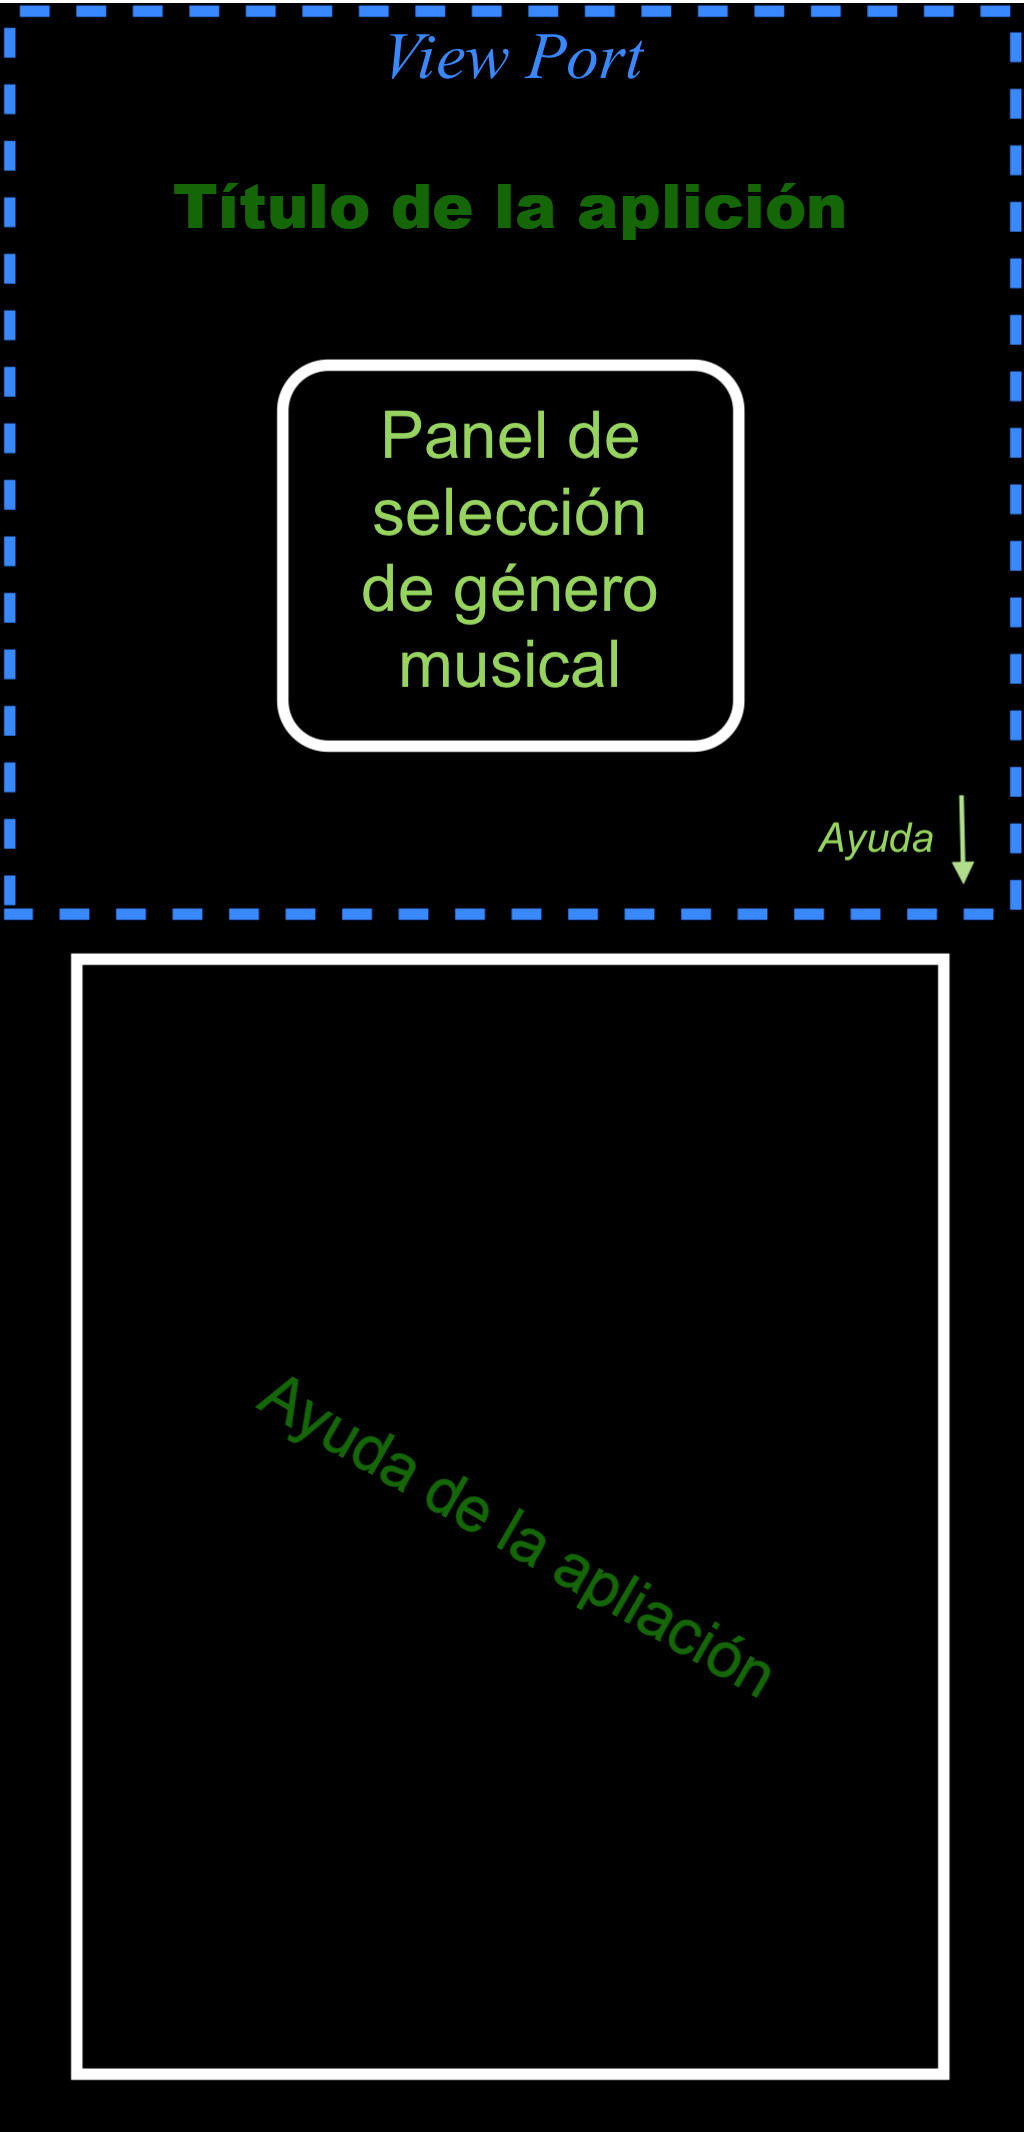
\includegraphics[width=0.35\textwidth]{images/panel_seleccion.png}
          \label{fig:pantalla-seleccion}}
      \subfigure[Pantalla de descarga y valoración.]{
        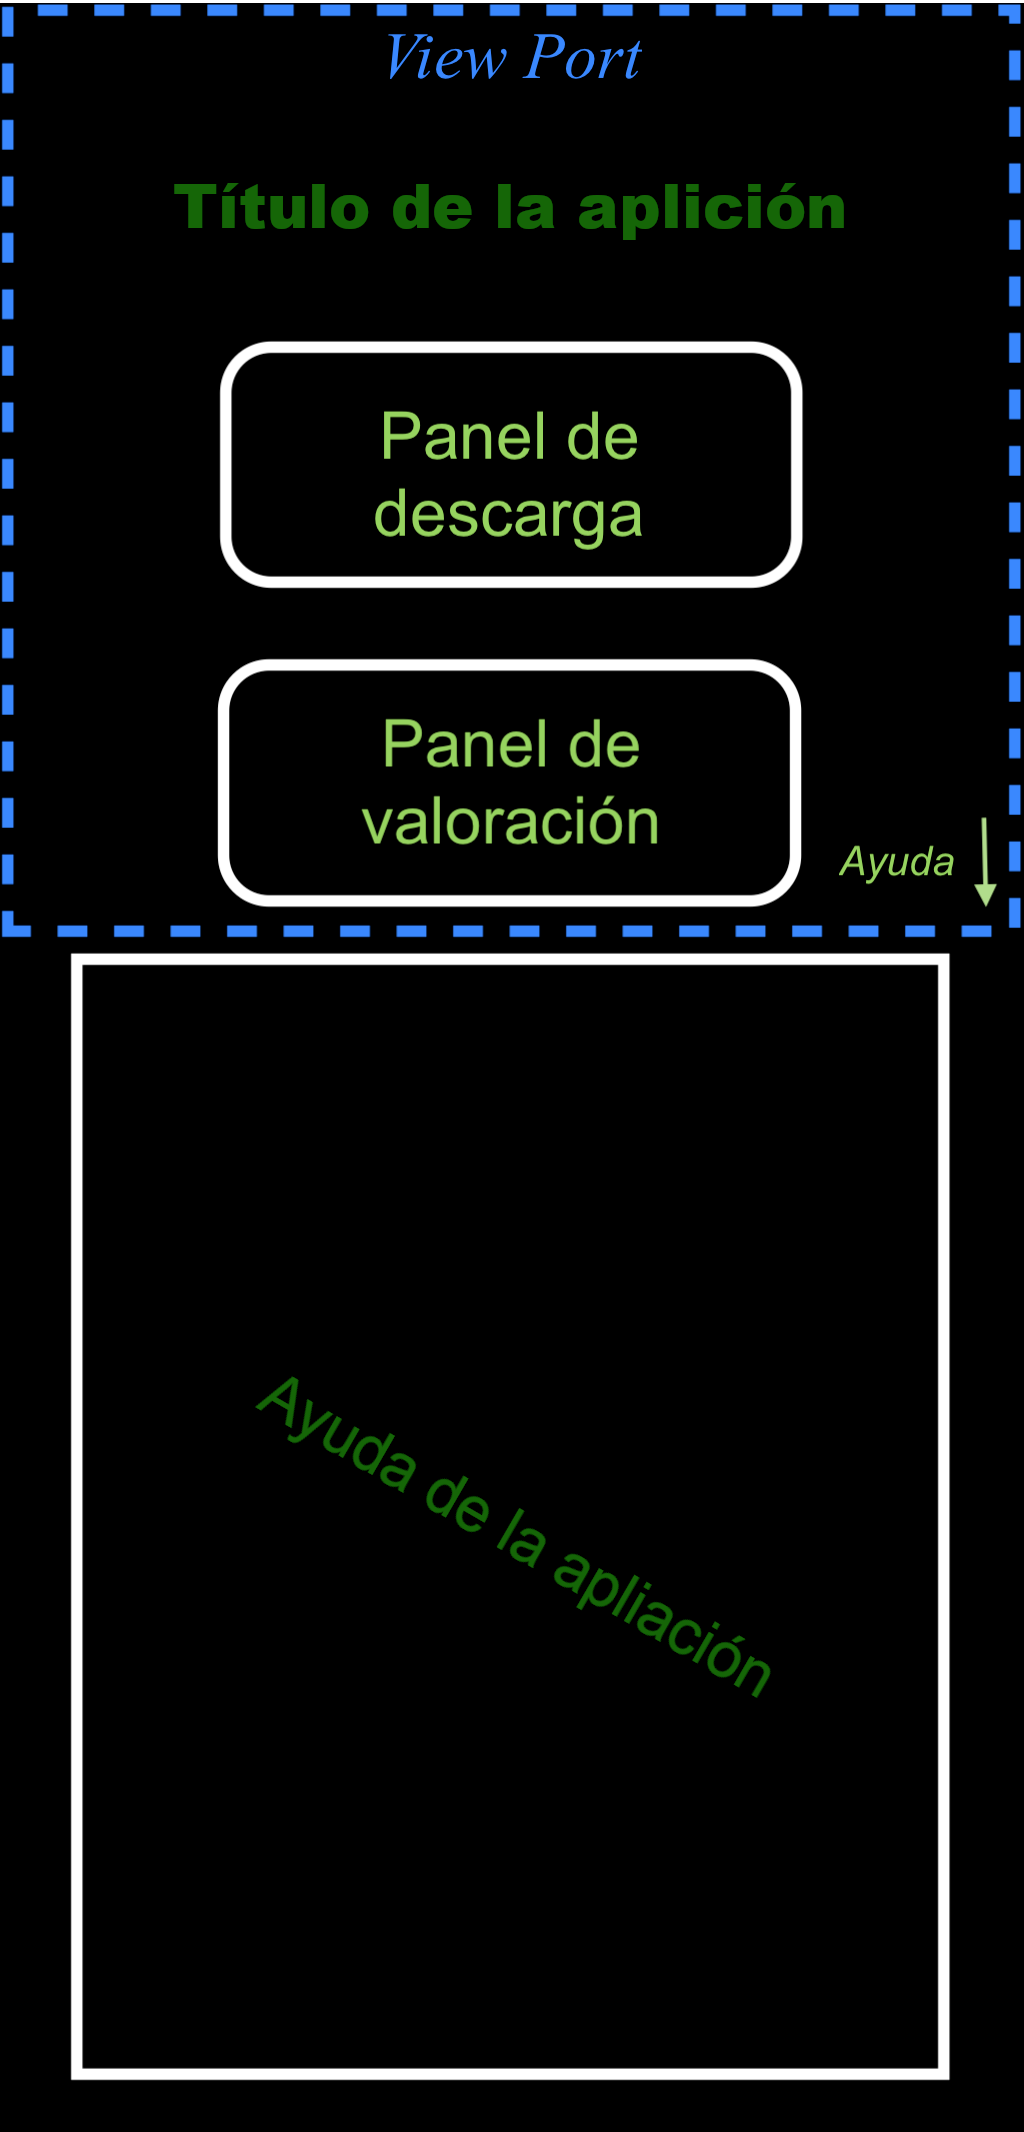
\includegraphics[width=0.35\textwidth]{images/panel-descarga-valoracion.png}
          \label{fig:pantalla-descarga}}
      \caption{Diseño de paneles de pantalla.}
      \label{fig:diseno-panales}
    \end{center}
  \end{figure}